
\documentclass[11pt,a4paper]{report}

\usepackage[utf8]{inputenc}
\usepackage[T1]{fontenc}
\usepackage{lmodern}
\usepackage[a4paper,margin=25mm]{geometry}
\usepackage{graphicx}
\usepackage{booktabs}
\usepackage{longtable}
\usepackage{array}
\usepackage{amsmath}
\usepackage{hyperref}
\usepackage{xcolor}
\usepackage{enumitem}
\usepackage{listings}
\usepackage{float}
\usepackage{caption}
\usepackage{microtype}
\graphicspath{{results/plots/}{../results/plots/}}

\hypersetup{
    colorlinks=true,
    linkcolor=black,
    urlcolor=blue,
    citecolor=black,
    pdftitle={AlgoBench: Algorithm Benchmarking and Profiling Suite},
    pdfauthor={IIT Dharwad CSE SSL Project Team}
}

\definecolor{codebg}{RGB}{246,247,243}
\definecolor{codegreen}{RGB}{75,105,58}
\lstset{
    basicstyle=\ttfamily\small,
    backgroundcolor=\color{codebg},
    frame=single,
    rulecolor=\color{black!15},
    breaklines=true,
    columns=fullflexible,
    keywordstyle=\color{codegreen}\bfseries,
    showstringspaces=false
}

\title{\Huge\bfseries AlgoBench\\[0.4em]
\Large Algorithm Benchmarking \& Profiling Suite}
\author{
    SSL Project\\[0.5em]
    Department of Computer Science and Engineering\\
    Indian Institute of Technology Dharwad\\[1em]
    \begin{tabular}{ll}
        CS25BT005 & Sorting and Searching\\
        CS25BT022 & Graph Algorithms\\
        CS25BT031 & Dynamic Programming and Matrix Algorithms\\
        CS25BT041 & Benchmarking and Profiling\\
        CS25BT051 & Dashboard and Integration
    \end{tabular}
}
\date{November 2026}

\begin{document}
\maketitle
\pagenumbering{roman}
\tableofcontents
\clearpage
\pagenumbering{arabic}

\chapter*{Abstract}
\addcontentsline{toc}{chapter}{Abstract}
Algorithm implementations are often studied through their asymptotic time
complexities, but observed performance also depends on input characteristics,
implementation choices, memory allocation, and runtime overhead. AlgoBench is
a Python-based algorithm benchmarking and profiling suite with a Streamlit
dashboard. It allows users to select algorithms, generate reproducible input
datasets, execute repeated measurements, inspect memory usage and profiling
reports, and compare performance as input size changes.

The project integrates sixteen implementations across sorting, searching,
graph algorithms, dynamic programming, and matrix multiplication. A reusable
benchmark engine measures function execution time using
\texttt{time.perf\_counter()}, estimates additional Python allocations using
\texttt{tracemalloc}, and optionally profiles function-level costs using
\texttt{cProfile} and \texttt{pstats}. CSV files provide persistent experiment
history, while GNUplot scripts prepare runtime and memory visualizations.

The unified automated test suite reports 158 passing pytest cases and 64
subtests in the integration environment. The dashboard was also exercised on
the project computer across all five domains. This report includes the CSV
measurements and GNUplot runtime and memory figures produced during those
local experiments. The measurements are specific to the recorded Windows and
CPython environment and should not be interpreted as universal timings.

\chapter{Introduction}

\section{Problem Statement}
Students commonly implement algorithms and compare them by theoretical
complexity. However, theoretical bounds alone do not show how implementations
behave for particular datasets or on a real execution environment. Two
algorithms with the same asymptotic complexity may have different constant
factors and memory demands. An algorithm may also behave differently on
random, sorted, reverse-sorted, sparse, or dense inputs.

A repeatable way is therefore needed to generate controlled datasets, execute
algorithms under consistent measurement conditions, inspect bottlenecks, and
visualize the observed results.

\section{Proposed Solution}
AlgoBench provides a single interface for configuring algorithm experiments.
It connects algorithm implementations and dataset generators to a generic
benchmark engine. The dashboard presents timing statistics, memory estimates,
profile reports, CSV history, and comparison charts.

\section{Objectives}
\begin{enumerate}[leftmargin=2em]
    \item Implement and organize algorithms from five computational domains.
    \item Generate deterministic datasets using configurable random seeds.
    \item Measure execution time over repeated trials.
    \item Measure additional Python memory allocations separately from timing.
    \item Use profiling tools to identify expensive functions.
    \item Compare observed performance over multiple input sizes.
    \item Provide CSV storage, history browsing, and runtime/memory plotting.
    \item Demonstrate modular development through Git, tests, Bash scripts, and a Makefile.
\end{enumerate}

\section{Scope}
The current implementation supports sixteen algorithm variants in five
categories. It focuses on reproducible Python experiments. Native profiling
support is included as an optional gprof demonstration for C programs; it is
separate from Python function profiling.

\chapter{System Design}

\section{High-Level Architecture}
The application follows a modular pipeline:

\begin{enumerate}
    \item \textbf{Streamlit dashboard:} accepts the user's category, algorithm,
    dataset, trial, seed, memory, and profiling choices.
    \item \textbf{Algorithm registry:} maps dashboard labels to Python callables
    and prepares the correct positional arguments.
    \item \textbf{Dataset generators:} create reproducible arrays, graphs,
    strings, item lists, and matrices.
    \item \textbf{Benchmark engine:} invokes registered callables and records
    timing, memory, and profiling metadata.
    \item \textbf{Storage and visualization:} writes CSV files, prepares
    GNUplot data, and displays comparison charts and history.
\end{enumerate}

\section{Project Modules}
\begin{longtable}{p{0.25\textwidth}p{0.65\textwidth}}
\toprule
\textbf{Module} & \textbf{Responsibility}\\
\midrule
\texttt{algorithms/} & Sorting, searching, graph, dynamic programming, and matrix implementations.\\
\texttt{data\_generation/} & Reproducible graph, string, and matrix datasets; array and item datasets are prepared by the registry.\\
\texttt{benchmarking/} & Algorithm registry, benchmark engine, timer, memory profiler, cProfile, and gprof integration.\\
\texttt{visualization/} & Streamlit charts and GNUplot data/plot generation.\\
\texttt{tests/} & Unit, generator, benchmark-engine, and integration tests.\\
\texttt{scripts/} & Bash helpers for running the app, tests, and GNUplot.\\
\texttt{reports/} & LaTeX report and Beamer source.\\
\bottomrule
\end{longtable}

\section{Algorithm Catalogue}
\begin{longtable}{p{0.18\textwidth}p{0.37\textwidth}p{0.34\textwidth}}
\toprule
\textbf{Domain} & \textbf{Algorithms} & \textbf{Representative time complexity}\\
\midrule
Sorting & Quick Sort, Merge Sort, Heap Sort, Insertion Sort &
Quick Sort: average $O(n\log n)$, worst $O(n^2)$; Merge/Heap: $O(n\log n)$; Insertion: average/worst $O(n^2)$.\\
Searching & Linear Search, Binary Search, Hash Table Lookup &
$O(n)$; $O(\log n)$ on ascending-sorted input; average $O(1)$ lookup.\\
Graph & Dijkstra, Bellman--Ford, BFS &
$O((V+E)\log V)$; $O(VE)$; $O(V+E)$.\\
Dynamic Programming & LCS memoization/tabulation; 0/1 Knapsack memoization/tabulation &
LCS: $O(mn)$; Knapsack: $O(nW)$.\\
Matrix & Standard Multiplication, Strassen Multiplication &
$O(n^3)$; approximately $O(n^{2.807})$ for square matrices.\\
\bottomrule
\end{longtable}

\section{Dataset Design}
The dataset generator uses a supplied seed to make experiments reproducible.

\begin{itemize}
    \item Sorting supports random, sorted, reverse-sorted, and nearly-sorted arrays.
    \item Searching supports successful and unsuccessful queries. When Binary
    Search is included in a comparison, the shared collection is made ascending-sorted.
    \item Graph experiments use connected, undirected weighted graphs with sparse or dense topology.
    \item LCS receives a pair of generated strings. Knapsack receives weights,
    values, and a capacity derived from the item count.
    \item Matrix algorithms receive the same pair of compatible square matrices
    for a given size and seed.
\end{itemize}

BFS reports shortest unweighted edge-count distances and ignores graph edge
weights. Dijkstra and Bellman--Ford use the positive edge weights generated by
the dashboard dataset factory.

\chapter{Benchmarking and Profiling Methodology}

\section{Runtime Measurement}
The benchmark engine uses Python's monotonic high-resolution performance
counter:
\begin{lstlisting}[language=Python]
start = time.perf_counter()
result = algorithm(*prepared_args)
elapsed = time.perf_counter() - start
\end{lstlisting}

An untimed warm-up call is performed before the timed trials. For each
algorithm and dataset, the engine records:
\begin{itemize}
    \item average execution time,
    \item median execution time,
    \item minimum and maximum execution time,
    \item standard deviation, and
    \item individual raw trial timings in the in-memory result.
\end{itemize}

Dataset generation and input preparation/copying occur outside the timed
interval. The measurement therefore represents the algorithm call itself.

\section{Memory Measurement}
Memory is measured separately using \texttt{tracemalloc}. The recorded value
is peak additional traced Python allocation in KiB during one algorithm call.
It is not the total RAM usage of the Python process. Running memory tracing
inside timed trials would distort runtime measurements, so the engine uses a
separate memory execution.

\section{Function Profiling}
The engine optionally uses \texttt{cProfile} and \texttt{pstats} to collect
function call counts, self time, cumulative time, and a textual report. Profile
runs are separate from timing trials. The dashboard profiles the largest
selected input size for each chosen algorithm to keep the experiment practical.

The optional \texttt{gprof\_profiler.py} module demonstrates profiling of
native C programs compiled with \texttt{gcc -pg}. This is distinct from
\texttt{cProfile}, which profiles Python functions.

\section{CSV Schema}
Each saved row includes timestamp, category, algorithm, input size, input
type, trial count, average/median/minimum/maximum time, standard deviation,
peak memory measurement, seed, and notes. The memory unit is KiB and runtime
units are seconds.

\section{GNUplot}
The GNUplot runner reads the CSV schema, pivots rows by category and input
type, prepares tab-separated \texttt{.dat} files, and invokes runtime and
memory plot scripts. Preparing data files does not require GNUplot; rendering
PNG plots requires the GNUplot executable to be installed and available on
the system \texttt{PATH}.

\chapter{Implementation}

\section{Dashboard Workflow}
The Run Benchmark page validates the selection and provides practical input
size ranges. Users may run one size or enable a scaling experiment over
multiple sizes. A progress indicator is updated after each algorithm-size
job. The resulting rows are stored in \texttt{results/} as a timestamped CSV.

The Compare Results page displays metrics and a runtime chart and provides
CSV download and GNUplot actions. The Profiler page shows the latest
cProfile summaries and saved reports. The History page loads experiment CSV
files saved in previous sessions.

\section{Benchmark Engine Interface}
The engine is algorithm-agnostic. A callable is registered under a category
and display name, and input data is passed as either a single argument or a
tuple of positional arguments.

\begin{lstlisting}[language=Python]
engine = create_default_engine(results_dir="results")
row = engine.run(
    "Sorting",
    "Merge Sort",
    dataset,
    input_size=1000,
    input_type="Random",
    trials=5,
    measure_memory=True,
    profile=True,
    seed=42,
)
\end{lstlisting}

This separation allows algorithm implementations to be integrated without
placing algorithm-specific logic inside the benchmark engine.

\section{Project Automation}
The repository includes Bash scripts for running the Streamlit application,
running tests, and generating GNUplot plots. A Makefile provides targets for
installation, app execution, testing, plotting, and cache cleanup.

\chapter{Testing and Validation}

\section{Automated Test Coverage}
The merged test suite includes tests for algorithm correctness, input
validation, dataset reproducibility, benchmark timing, memory profiling,
cProfile output, CSV persistence, GNUplot data preparation, algorithm
registration, and execution through the common engine interface.

\begin{center}
\begin{tabular}{lr}
\toprule
\textbf{Validation item} & \textbf{Observed result}\\
\midrule
Python source files syntax-checked & 35\\
Unified pytest cases passed & 158\\
Subtests passed & 64\\
Direct smoke test of registered algorithms & 16 / 16\\
GNUplot data-file preparation smoke test & Passed\\
\bottomrule
\end{tabular}
\end{center}

The test results above are from the integration environment used to assemble
the project. The Streamlit browser interface was launched on the project computer. All
five algorithm domains were run through the dashboard, CSV files were saved,
and GNUplot runtime and memory PNGs were rendered for each domain.

\section{Manual Validation Checklist}
\begin{enumerate}
    \item Start the application using \texttt{streamlit run app.py}.
    \item Enter the dashboard through the animated logo landing page.
    \item Switch Bright and Dark themes.
    \item Run one small experiment from each of the five categories.
    \item Run a scaling experiment with at least three input sizes.
    \item Verify that each run creates a CSV in \texttt{results/}.
    \item Open Compare Results, Profiler, and History.
    \item Render GNUplot runtime and memory PNG plots for all five domains.
\end{enumerate}

\chapter{Results and Discussion}

\section{Experimental Environment and Protocol}
The benchmark evidence was generated on the project team's Windows computer.
The profiler report paths identify CPython 3.14; the CPU model and hardware
configuration were not included in the supplied evidence, so they are not
reported here. Each datapoint is the average of five timed trials. The
benchmark engine performs an untimed warm-up and measures the algorithm call
separately from dataset construction and input preparation. Memory is measured
in a separate \texttt{tracemalloc} execution and is reported as peak additional
traced Python allocation in KiB.

The scaling datasets included random integer arrays for sorting, successful
queries over ascending-sorted collections for searching, sparse connected
weighted graphs for graph algorithms, random strings and random item sets for
dynamic programming, and random square matrices for matrix multiplication.
All comparisons use the input-size conventions shown in the dashboard. In
particular, the searching experiment excludes hash-table construction from
the timed Hash Table Lookup operation, and BFS measures unweighted
edge-count distance rather than weighted shortest paths.

\section{Sorting}
Four sorting algorithms were measured on random arrays of 100, 500, 1,000,
2,000, and 5,000 elements. Table~\ref{tab:sorting-results} reports average
runtime in milliseconds.

\begin{table}[H]
\centering\small
\caption{Sorting runtime by input size (milliseconds; five trials per point).}
\label{tab:sorting-results}
\begin{tabular}{rrrrr}
\toprule
$n$ & Quick Sort & Merge Sort & Heap Sort & Insertion Sort\\
\midrule
100 & 0.249 & 0.397 & 0.416 & 0.274\\
500 & 0.941 & 1.858 & 1.404 & 5.469\\
1,000 & 1.890 & 3.480 & 3.890 & 34.258\\
2,000 & 5.563 & 6.146 & 8.891 & 115.178\\
5,000 & 12.839 & 18.572 & 26.990 & 540.030\\
\bottomrule
\end{tabular}
\end{table}

At 5,000 elements, Insertion Sort took approximately 0.540 seconds, compared
with 0.0128 seconds for Quick Sort. This is consistent with the expected
quadratic growth of insertion sort on random input, while the other three
implementations grew more slowly over the tested range. Quick Sort was the
fastest of the four in the largest-size run. These are observed implementation
results on one machine, not guarantees for every input distribution.

\begin{figure}[H]
\centering
\begin{minipage}{0.49\textwidth}\centering
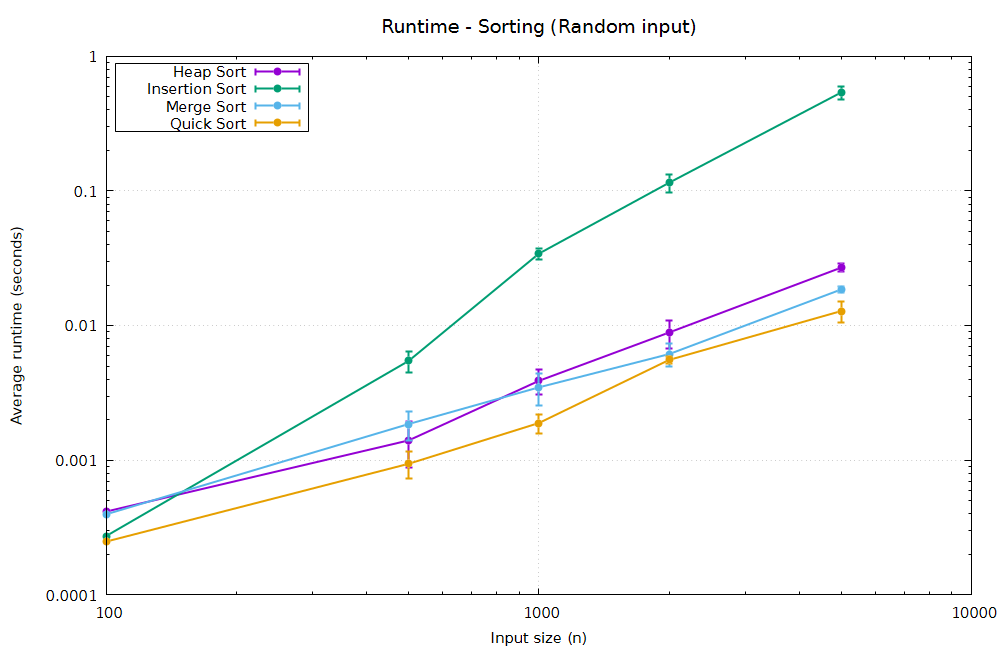
\includegraphics[width=\linewidth]{Sorting_Random_runtime.png}
\caption{Sorting runtime scaling.}\label{fig:sorting-runtime}
\end{minipage}\hfill
\begin{minipage}{0.49\textwidth}\centering
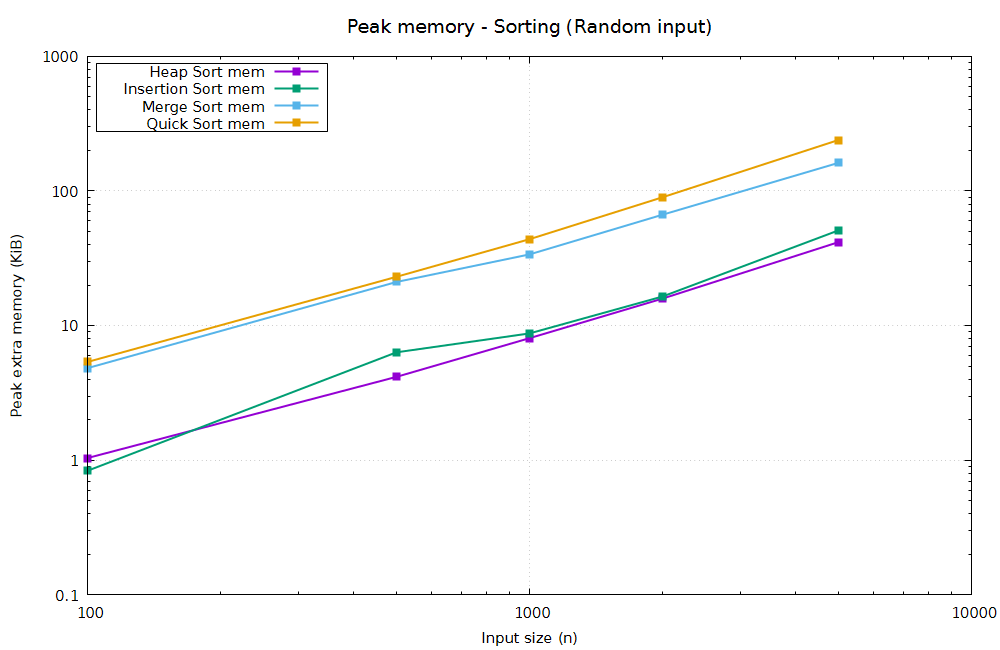
\includegraphics[width=\linewidth]{Sorting_Random_memory.png}
\caption{Sorting peak additional memory.}\label{fig:sorting-memory}
\end{minipage}
\end{figure}

\section{Searching}
Linear Search, Binary Search, and Hash Table Lookup were compared for
successful queries on ascending-sorted collections of 1,000, 5,000, 10,000,
and 50,000 elements. Table~\ref{tab:search-results} shows average runtime in
milliseconds.

\begin{table}[H]
\centering\small
\caption{Searching runtime by collection size (milliseconds; five trials).}
\label{tab:search-results}
\begin{tabular}{rrrr}
\toprule
$n$ & Linear Search & Binary Search & Hash Table Lookup\\
\midrule
1,000 & 0.0901 & 0.0131 & 0.00538\\
5,000 & 0.3560 & 0.0117 & 0.00432\\
10,000 & 0.7300 & 0.0119 & 0.00526\\
50,000 & 3.2961 & 0.0148 & 0.00338\\
\bottomrule
\end{tabular}
\end{table}

Linear Search increased from about 0.090 ms at 1,000 elements to 3.296 ms at
50,000 elements. Binary Search remained around 0.012--0.015 ms, and the
measured hash lookup remained around 0.003--0.005 ms. The hash lookup result
covers lookup only; table construction is outside the timed operation.
The reported 0.0 KiB memory values for Binary Search and Hash Table Lookup
mean that no additional traced allocation was observed in that isolated call
at the recorded precision, not that these algorithms require zero total
memory.

\begin{figure}[H]
\centering
\begin{minipage}{0.49\textwidth}\centering
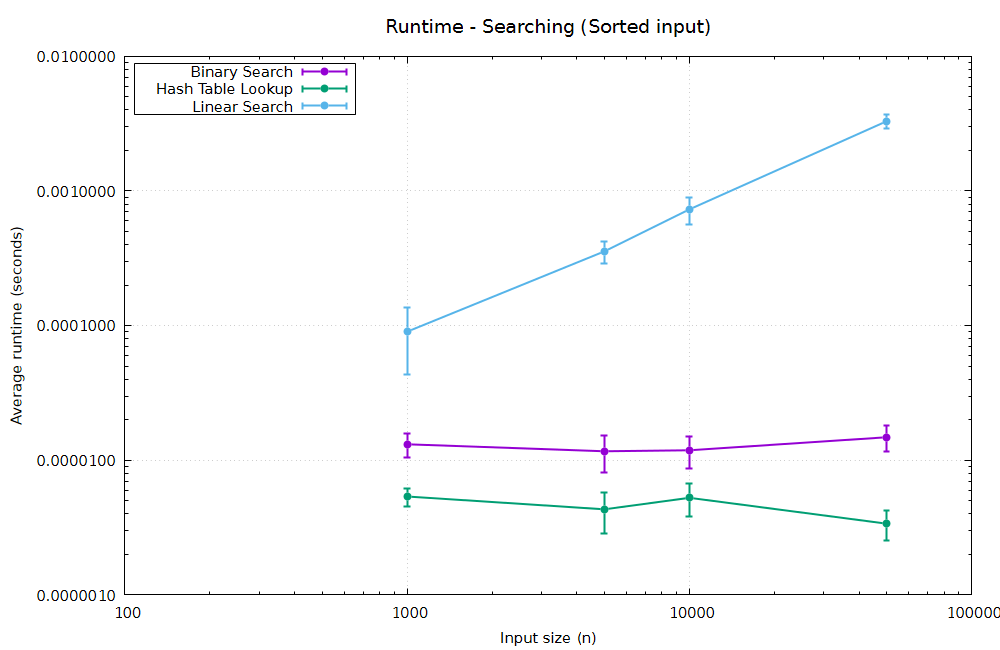
\includegraphics[width=\linewidth]{Searching_Sorted_runtime.png}
\caption{Searching runtime scaling.}\label{fig:search-runtime}
\end{minipage}\hfill
\begin{minipage}{0.49\textwidth}\centering
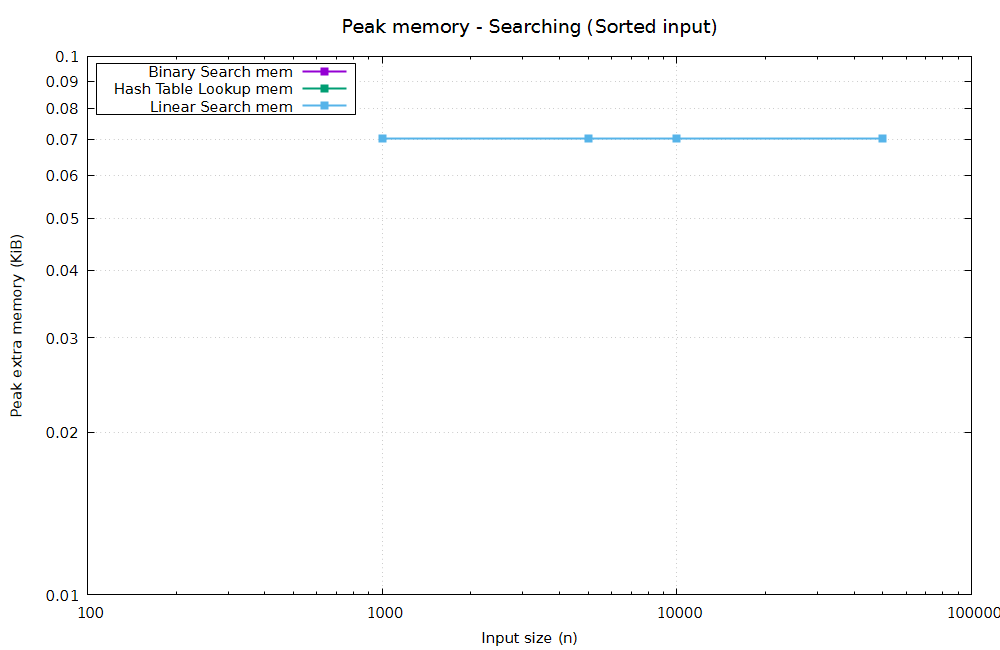
\includegraphics[width=\linewidth]{Searching_Sorted_memory.png}
\caption{Searching peak additional memory.}\label{fig:search-memory}
\end{minipage}
\end{figure}

\section{Graph Algorithms}
Dijkstra, Bellman--Ford, and BFS were tested on sparse connected weighted
graphs with 20, 50, 100, and 200 vertices. Each point represents five timed
trials. Table~\ref{tab:graph-results} reports milliseconds.

\begin{table}[H]
\centering\small
\caption{Sparse graph runtime by vertex count (milliseconds; five trials).}
\label{tab:graph-results}
\begin{tabular}{rrrr}
\toprule
Vertices & Dijkstra & Bellman--Ford & BFS\\
\midrule
20 & 0.110 & 0.141 & 0.134\\
50 & 0.190 & 0.678 & 0.136\\
100 & 0.324 & 0.839 & 0.231\\
200 & 0.781 & 1.051 & 0.535\\
\bottomrule
\end{tabular}
\end{table}

All three runtimes increased over the tested vertex counts. Bellman--Ford
was the slowest at 50, 100, and 200 vertices in this scaling run. Dijkstra
was faster than Bellman--Ford on the larger tested graphs. BFS was also fast,
but its result is not a like-for-like weighted shortest-path comparison:
BFS returns unweighted edge-count distances and ignores edge weights. The
50-vertex point has relatively high trial variability for Bellman--Ford, as
reflected by its recorded standard deviation, so the difference at that size
should be interpreted cautiously.

\begin{figure}[H]
\centering
\begin{minipage}{0.49\textwidth}\centering
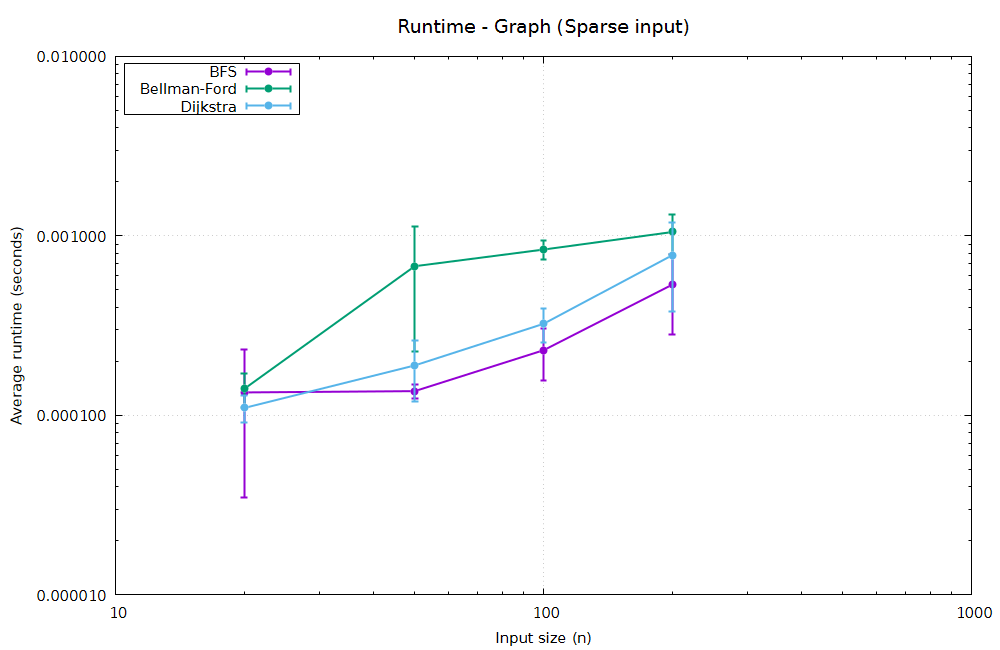
\includegraphics[width=\linewidth]{Graph_Sparse_runtime.png}
\caption{Sparse graph runtime scaling.}\label{fig:graph-runtime}
\end{minipage}\hfill
\begin{minipage}{0.49\textwidth}\centering
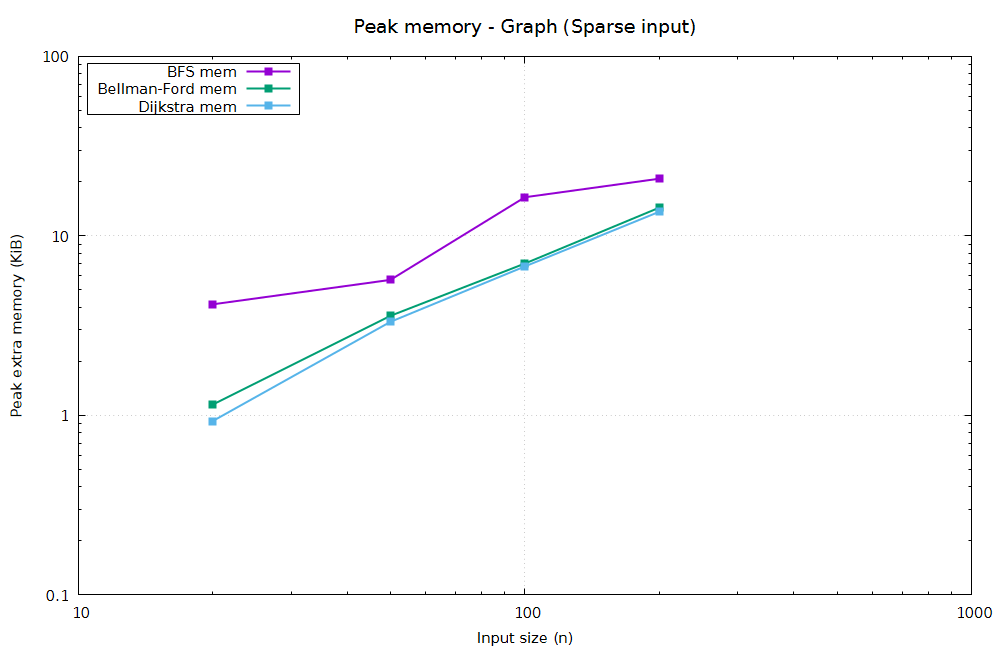
\includegraphics[width=\linewidth]{Graph_Sparse_memory.png}
\caption{Sparse graph peak additional memory.}\label{fig:graph-memory}
\end{minipage}
\end{figure}

\section{Dynamic Programming}
The dynamic-programming experiments were split into two workload families:
LCS on pairs of random strings and 0/1 Knapsack on random item sets. Both
families were measured at input sizes 10, 20, 40, 60, 80, and 100. Each
algorithm-size point contains five trials. Table~\ref{tab:dp-results} reports
average runtime in milliseconds.

\begin{table}[H]
\centering\small
\caption{Dynamic-programming runtime (milliseconds; five trials).}
\label{tab:dp-results}
\begin{tabular}{rrrrr}
\toprule
$n$ & LCS Memo. & LCS Tab. & Knapsack Memo. & Knapsack Tab.\\
\midrule
10  & 0.169 & 0.059 & 0.214 & 0.196\\
20  & 0.691 & 0.133 & 1.102 & 0.514\\
40  & 1.613 & 0.383 & 4.803 & 2.582\\
60  & 2.680 & 0.743 & 10.892 & 5.310\\
80  & 4.752 & 1.445 & 21.987 & 10.394\\
100 & 5.679 & 1.923 & 46.322 & 12.086\\
\bottomrule
\end{tabular}
\end{table}

For both LCS and Knapsack, tabulation was faster than memoization at the
larger tested sizes. At size 100, LCS tabulation took approximately 1.923 ms
versus 5.679 ms for memoization; Knapsack tabulation took 12.086 ms versus
46.322 ms for memoization. The memory measurements show the same direction
in these runs: at size 100, memoized Knapsack used about 7,072.8 KiB of peak
additional traced memory, while tabulation used about 805.8 KiB. The result
is workload- and implementation-dependent and does not establish that one
approach is always superior.

\begin{figure}[H]
\centering
\begin{minipage}{0.49\textwidth}\centering
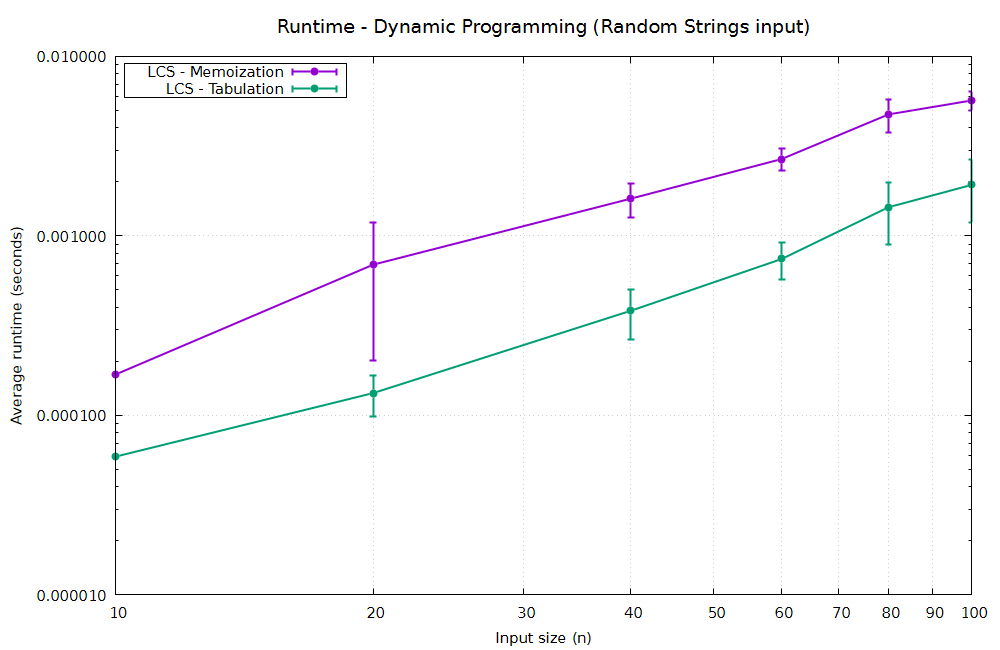
\includegraphics[width=\linewidth]{Dynamic_Programming_Random_Strings_runtime.png}
\caption{LCS runtime scaling.}\label{fig:lcs-runtime}
\end{minipage}\hfill
\begin{minipage}{0.49\textwidth}\centering
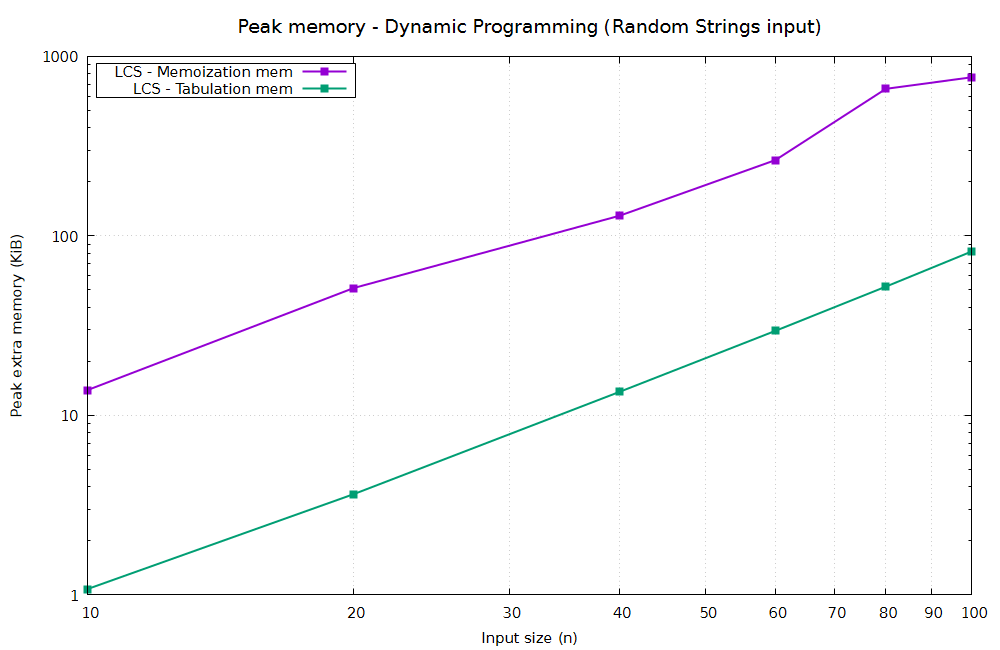
\includegraphics[width=\linewidth]{Dynamic_Programming_Random_Strings_memory.png}
\caption{LCS peak additional memory.}\label{fig:lcs-memory}
\end{minipage}
\end{figure}

\begin{figure}[H]
\centering
\begin{minipage}{0.49\textwidth}\centering
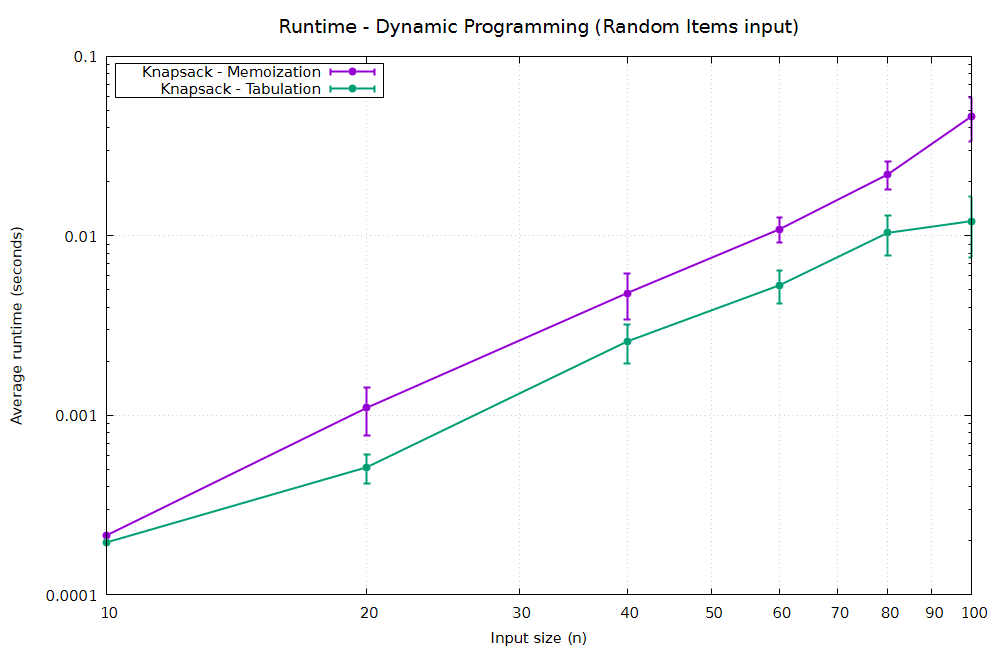
\includegraphics[width=\linewidth]{Dynamic_Programming_Random_Items_runtime.png}
\caption{Knapsack runtime scaling.}\label{fig:knapsack-runtime}
\end{minipage}\hfill
\begin{minipage}{0.49\textwidth}\centering
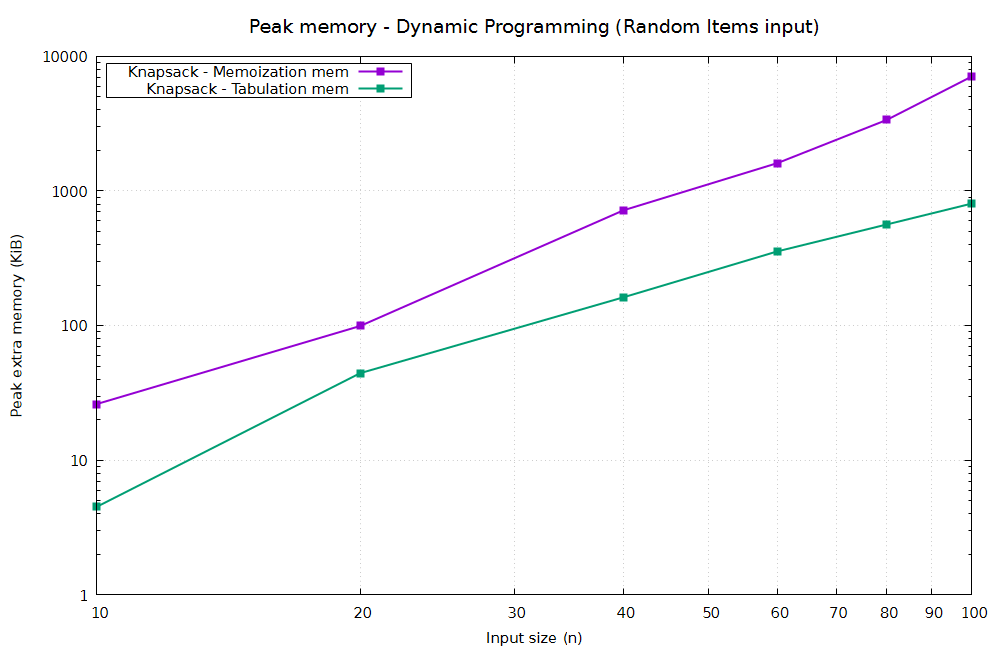
\includegraphics[width=\linewidth]{Dynamic_Programming_Random_Items_memory.png}
\caption{Knapsack peak additional memory.}\label{fig:knapsack-memory}
\end{minipage}
\end{figure}

\section{Matrix Multiplication}
Standard and Strassen multiplication were run on pairs of random square
matrices of dimensions 32, 64, and 128. Table~\ref{tab:matrix-results}
reports average runtime in milliseconds and peak additional traced memory in
KiB.

\begin{table}[H]
\centering\small
\caption{Matrix multiplication measurements (five trials per point).}
\label{tab:matrix-results}
\begin{tabular}{rrrrr}
\toprule
Dimension & Standard (ms) & Strassen (ms) & Standard mem. (KiB) & Strassen mem. (KiB)\\
\midrule
32  & 4.751 & 4.603 & 38.2 & 64.8\\
64  & 30.536 & 31.623 & 165.5 & 656.6\\
128 & 249.948 & 272.290 & 650.7 & 2,533.3\\
\bottomrule
\end{tabular}
\end{table}

Strassen was marginally faster at dimension 32, but standard multiplication
was faster at 64 and 128 in these measurements. At dimension 128, Strassen
was about 9\% slower and used approximately 3.9 times the peak additional
traced memory. This is a useful practical crossover observation: the lower
asymptotic exponent of Strassen does not guarantee a speedup at the modest
matrix sizes tested, especially when recursion and temporary matrix
allocations have non-trivial overhead. Larger dimensions would be required
to locate a crossover point for this implementation and machine.

\begin{figure}[H]
\centering
\begin{minipage}{0.49\textwidth}\centering
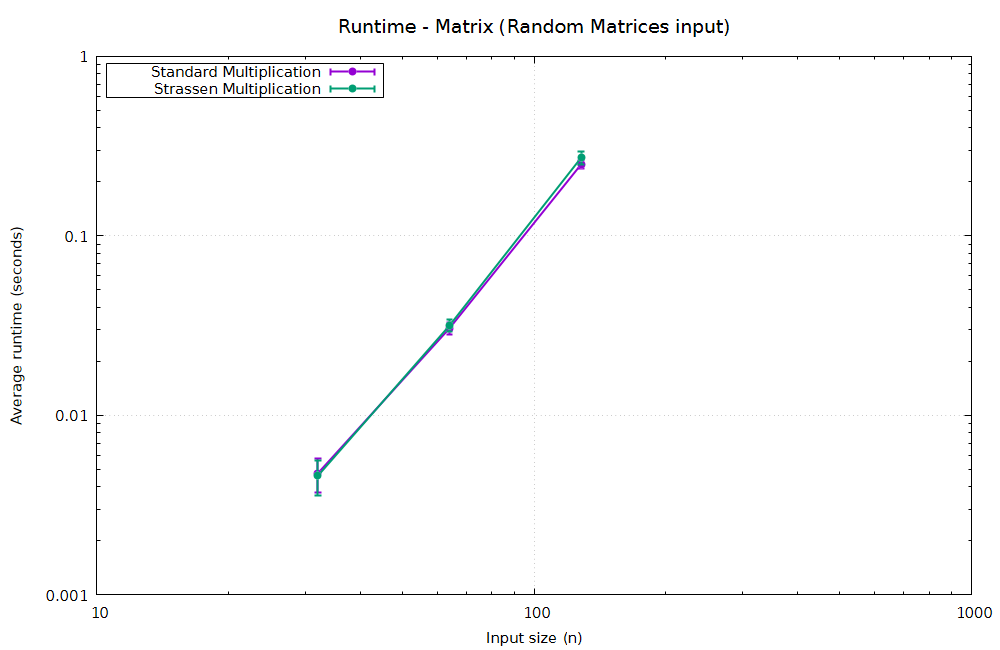
\includegraphics[width=\linewidth]{Matrix_Random_Matrices_runtime.png}
\caption{Matrix multiplication runtime scaling.}\label{fig:matrix-runtime}
\end{minipage}\hfill
\begin{minipage}{0.49\textwidth}\centering
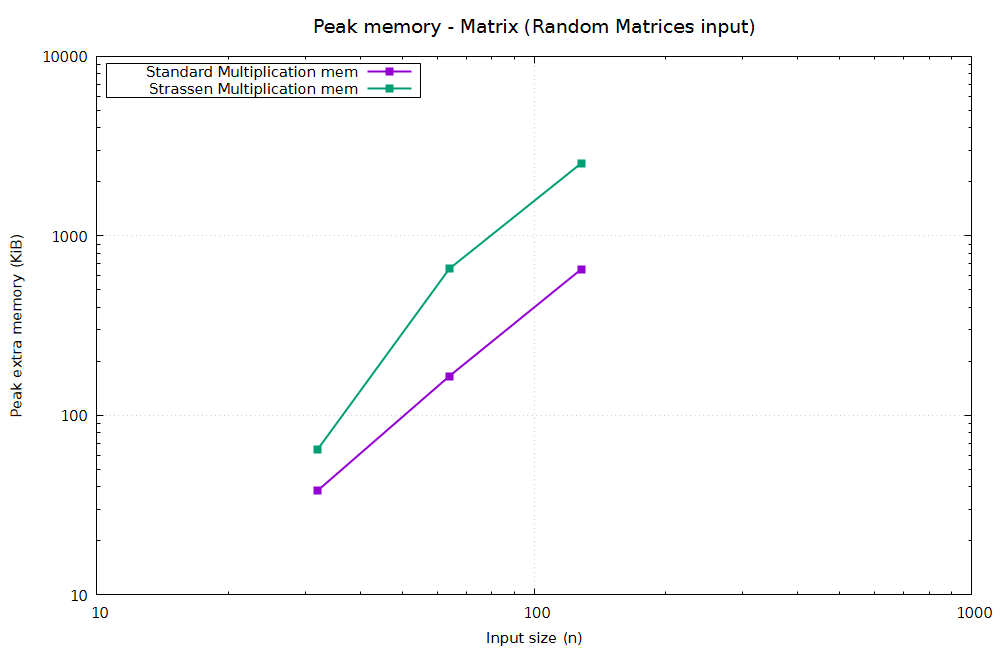
\includegraphics[width=\linewidth]{Matrix_Random_Matrices_memory.png}
\caption{Matrix multiplication peak additional memory.}\label{fig:matrix-memory}
\end{minipage}
\end{figure}

\section{Profiler Observations}
The supplied \texttt{cProfile}/\texttt{pstats} text reports show algorithm
functions and, in some captures, activity from the Streamlit host process.
Examples of algorithm-level observations include:
\begin{itemize}
    \item Quick Sort at input size 5,000 recorded 5,971 recursive \texttt{sort}
    calls (with one outer invocation) and approximately 0.020 seconds
    cumulative time in the profiled algorithm call.
    \item Knapsack memoization at input size 100 recorded 45,463 recursive
    \texttt{solve} calls (including the outer call) and 44,869 calls to
    \texttt{max}, illustrating the repeated state evaluation and comparison
    activity in that implementation.
    \item The Strassen profile at dimension 128 recorded 57 calls to
    \texttt{\_strassen\_recursive}; it also showed repeated base-case calls
    to standard multiplication and matrix addition/subtraction helpers.
\end{itemize}

\textbf{Profiler caveat:} some profile files include Streamlit watcher,
asyncio, and background-thread events in their cumulative-time ordering.
For example, the Insertion Sort profile at size 5,000 includes substantial
watcher and event-loop activity alongside the \texttt{insertion\_sort}
function. Therefore, the profile tables are useful for inspecting function
calls, but cumulative times from a Streamlit-hosted profile should not be
attributed wholly to the selected algorithm. A future improvement would be
to run profiling in a separate worker process to isolate application-server
overhead.

\section{Overall Findings}
Across the supplied scaling experiments, the observed trends broadly align
with the expected complexity patterns: Insertion Sort and Linear Search
increase more sharply with input size than their more efficient alternatives;
LCS and Knapsack runtimes rise with their workload sizes; and graph runtimes
increase as vertices are added. The matrix experiment did not reach a size at
which Strassen outperformed standard multiplication. The plots also show
that time and memory are separate dimensions: an implementation that is
competitive in runtime may allocate more temporary memory.

These results are five-trial measurements from one Windows/CPython 3.14
environment. Small timings, especially microsecond-scale search operations,
are sensitive to system scheduling and measurement overhead. They should be
used as a reproducible project demonstration, not as hardware-independent
performance claims.

\chapter{Limitations and Future Work}

\section{Current Limitations}
\begin{itemize}
    \item GNUplot rendering requires a separately installed system executable.
    \item \texttt{tracemalloc} measures traced Python allocations, not all
    process memory or native allocations.
    \item The native gprof example requires a supported GCC/gprof environment;
    Windows users are advised to use WSL.
    \item Benchmark values are machine- and workload-dependent.
    \item The dashboard's browser-level interaction should be rechecked on
    the final presentation machine, since browser dimensions and deployment
    environments can differ from the development laptop.
\end{itemize}

\section{Future Work}
Potential extensions include additional algorithm families, more dataset
distributions, persistent profile browsing by experiment, exportable PDF
benchmark reports, native C/C++ algorithm implementations, and automated
benchmark comparisons over multiple machines.

\chapter{Conclusion}
AlgoBench combines algorithm implementations, reproducible dataset generation,
a reusable benchmark engine, memory measurement, function profiling, CSV
history, and visualization in one modular application. Its registry-driven
design keeps algorithms separate from benchmarking mechanics and allows the
dashboard to invoke different algorithms through a common interface. The
integrated tests validate all sixteen registered implementations through the
benchmark engine. The final demonstration should record fresh machine-specific
measurements and show the full dashboard workflow.

\chapter*{Team Contributions}
\addcontentsline{toc}{chapter}{Team Contributions}
\begin{longtable}{p{0.18\textwidth}p{0.72\textwidth}}
\toprule
\textbf{Member} & \textbf{Contribution}\\
\midrule
CS25BT005 & Sorting and searching implementations and their unit tests.\\
CS25BT022 & Graph algorithms, graph dataset generator, and tests.\\
CS25BT031 & LCS, Knapsack, matrix multiplication, string/matrix generators, and tests.\\
CS25BT041 & Generic benchmark engine, runtime/memory measurement, cProfile/gprof support, GNUplot scripts, and engine tests.\\
CS25BT051 & Streamlit dashboard, integration, result browsing, automation, and final project packaging.\\
\bottomrule
\end{longtable}

\chapter*{References}
\addcontentsline{toc}{chapter}{References}
\begin{enumerate}
    \item T. H. Cormen, C. E. Leiserson, R. L. Rivest, and C. Stein,
    \textit{Introduction to Algorithms}, 4th ed., MIT Press, 2022.
    \item Python Software Foundation, \textit{Python Documentation},
    \url{https://docs.python.org/}.
    \item Streamlit, \textit{Streamlit Documentation},
    \url{https://docs.streamlit.io/}.
    \item GNU Project, \textit{GNUplot Documentation},
    \url{https://www.gnuplot.info/documentation.html}.
\end{enumerate}

\chapter*{AI Tool Usage Declaration}
\addcontentsline{toc}{chapter}{AI Tool Usage Declaration}
The team used ChatGPT for assistance with integration planning, dashboard
and benchmark-engine integration, debugging guidance, and drafting the project
report and presentation. Claude was used to produce a review and testing report
for the integrated application. The team ran the application locally across
the five algorithm domains and collected the CSV measurements and GNUplot
figures included in this report. The team remains responsible for reviewing
the complete submitted code, understanding the algorithms and measurement
methodology, and being able to explain all AI-assisted changes during the
project evaluation. Each member should verify the description above and
amend it if any additional AI assistance needs to be declared under the course
instructions.

\end{document}
